\chapter{Cybersecurity Risk Analysis}

\begin{figure}[H]
\centering
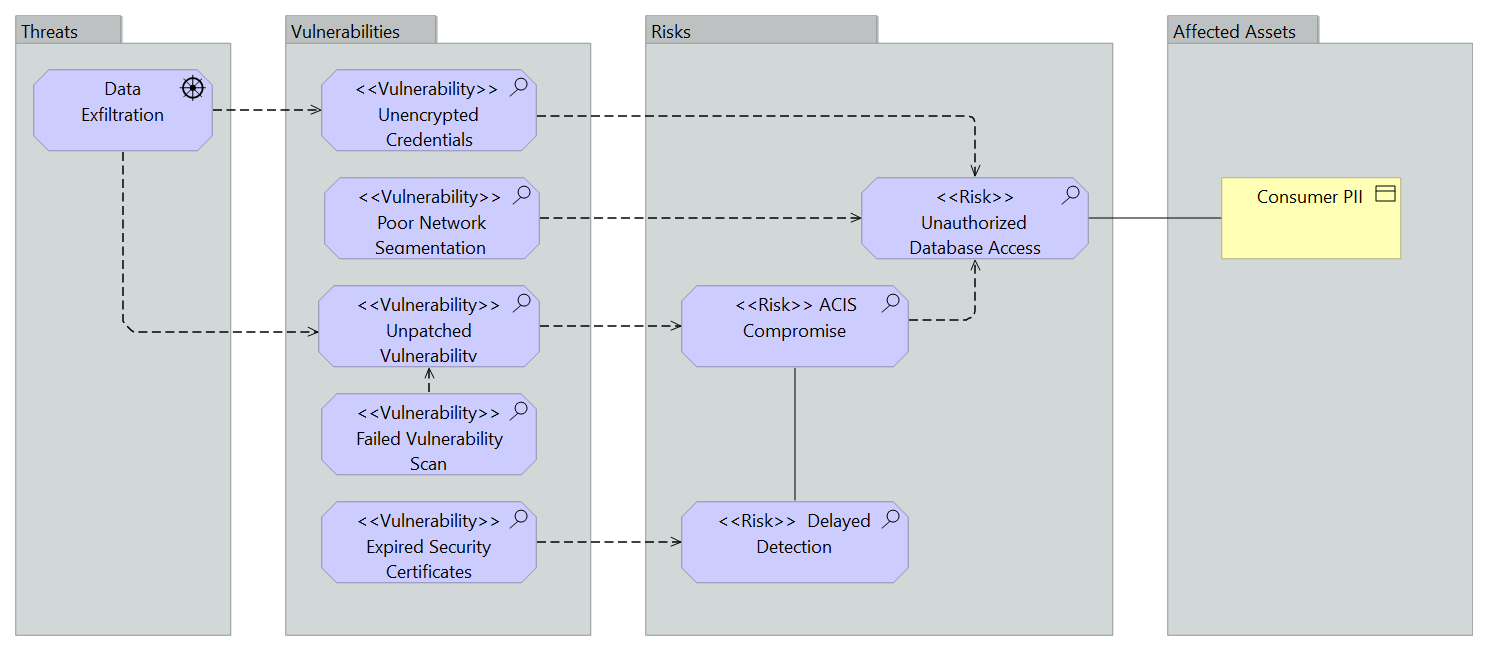
\includegraphics[width=1\linewidth]{images/risk-view.png}
\caption{Risk view.}
\end{figure}

The given view identifies main threats, vulnerabilities, risks and affected assets that were in place when the incident occurred and how they are connected to each other.
\newline
The primary threat is represented as \textbf{data exfiltration} as the consumer dispute process handled consumer reports which contain highly sensitive consumer information.
\newline
Firstly, the view identifies \textbf{unencrypted credentials} and \textbf{poor network segmentation} as vulnerabilities. Once the attackers initially breached the environment, they found a file containing unencrypted credentials that could be used to access Equifax's databases. Additionally, a poor network segmentation led to the attackers being able to perform query on said databases as they were in the same network as the databases used by ACIS.
\newline
Second, although a patch for the vulnerability CVE-2017-5638 was available, it has not been applied to the applications that needed the patch. In particular, the solution used by Equifax to detect vulnerabilities in their applications failed to identify the systems that needed patch. This led to the attackers exploiting the vulnerability to compromise ACIS in order to move to Equifax's databases.
\newline
Lastly, the security certificate for monitoring network traffic in the ACIS environment has been expired for 19 months prior to the incident which led to the compromise of ACIS being undetected until the certificate got renewed.
\newline
These vulnerabilities were responsible for the compromise of ACIS, it's delayed detection and subsequent unauthorized database access which contained the consumer's PII that the attackers exfiltrated.